% Copyright (C) 2011 Thomas L. Kula
% All Rights Reserved
%
% See the file LICENSE for license terms.
\documentclass[12pt]{article}
\usepackage{graphicx}
\usepackage{rotating}
\usepackage{fix-cm}
\usepackage{multirow}
\setlength{\paperwidth}{5.5in}
\setlength{\paperheight}{8.5in}
\setlength{\textheight}{7.45in}
\setlength{\topmargin}{-1.0in}
\setlength{\oddsidemargin}{-0.5in}
\setlength{\evensidemargin}{-0.5in}
\setlength{\textwidth}{4.0in}
\setlength{\parindent}{0in}
\setlength{\parskip}{3mm}
\usepackage[print]{booklet} \nofiles
\source{\magstep0}{5.5in}{8.5in}
\target{\magstep0}{11in}{8.5in}
\setpdftargetpages
\pagestyle{empty}
\begin{document}


\begin{center}
{\fontsize{36}{48}\selectfont \textsc{Haiku a Day }}
\end{center}

\vspace*{3.5cm}

{\fontsize{20}{40}\selectfont 

A nascent springtime

A man's fancy turns towards

Long bicycle rides


}

\vspace*{5.0cm}
\begin{center}
{\large{Issue 69: March 2011}} \\[5mm]
{\fontsize{8}{8}\selectfont  \textsc{ St. Joshua Norton Press }} \\[1mm]
{\fontsize{6}{6}\selectfont Mathom House in Midtown \textbar The People's Republic of Ames }
\end{center}


\newpage

Haiku a Day is never late, nor is it early. It arrives precisely when it means to.  \\
--- Thomas

http://kula.tproa.net/had/ \\
kula@tproa.net

Download this and previous HADs at the website, so you can
print out your own (DIY, yeah!) or if you want me to send
you one, send me your address, and maybe a stamp if you
are feeling nice. Or send me something you've made ---
trades always appreciated, postcards are nice too.

\vfill

1 March 2011

Like desperate hands \\
Errant branches spring from earth \\
Straining for the sky

2 March 2011

Woke up too early \\
Brain is still off, not thinking \\
A fog of tired

3 March 2011

People cannot drive \\
Like idiots, dumbfounded \\
Two ton missiles

\newpage

4 March 2011

From behind my eye \\
Dull throbbing resonating \\
Ruining my day

5 March 2011

A green hat, bobbing, \\
Dashing past the front window \\
Disappears from sight

6 March 2011

Castles floating high \\
Soaring only from anchors \\
Buried in the ground

7 March 2011

A craving for peas \\
Delicate green orbs, tiny \\
Sweet bursts of flavor

8 March 2011

A mighty ocean \\
Bestrode by a titan tall \\
Boy plays in the mud

9 March 2011

Rock and roll music? \\
It is too loud. Soft music, \\
A nice polka, no?

10 March 2011

Beware, Tens of March \\
What, ides? What the hell are ides? \\
Where is that memo?


\newpage

11 March 2011

What's beyond that grove? \\
Over that hill? Down that path? \\
With walking you learn

12 March 2011

Why do you rumble? \\
You should be happy, tummy, \\
So why are you sad?

13 March 2011

Turn and turn again \\
In a tight spiral we go \\
Waiting in a line

14 March 2011

Numbers all lined up \\
Attempting to find order \\
In the data sea

15 March 2011

Cautiously, green buds \\
Emerge from brown earth, peeking \\
Is it the right time?

16 March 2011

From good comes evil \\
Wholesomeness plus deep fryer \\
Oh what have we wraught?

17 March 2011

Windows opening \\
Letting the first real Spring in \\
Breeze removes Winter

\newpage

18 March 2011

Ominous grumbles \\
Calling out from my tummy \\
Why are you so sad?

19 March 2011

Little old lady \\
Driving a tiny car --- zoom! \\
Gliding down the street

20 March 2011

Mega power nap \\
Four hours long --- impressive \\
Even I respect

21 March 2011

Thirty-six hours \\
Stuck inside my apartment \\
I'm glad to get out

22 March 2011

Tiny ice nuggets \\
Not even grains of rice size \\
Weak slush from above

23 March 2011

Infinite Tacos \\
Not just a buffet item \\
But a good band name

24 March 2011

I'm an idiot! \\
That box, my toe, late at night \\
Curse the sky above


\newpage

25 March 2011

My late night reading \\
Lately, technical papers \\
I dream protocols

26 March 2011

Long and winding path \\
As of now, barren and grey \\
But spring! Spring come soon

27 March 2011

Forgotten noodles \\
Did not get put in spring rolls \\
I'm an idiot

28 March 2011

Entropy for real \\
A neat stack of news papers \\
Meets a windy breeze

29 March 2011

Where the seasons go \\
Once anticipatory \\
Yet fleeting they go

30 March 2011

The bald sun, staring \\
Glaring sternly down on us \\
Unimpressed, snarky

31 March 2011

These pants shed cat hair \\
But I don't own a damn cat \\
Stupid static sucks

\newpage

\begin{center}
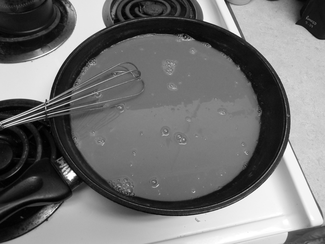
\includegraphics{coffee-gravy.png}

Coffee. Gravy. \\
{\tt kula.tproa.net/photos/2011/20110326-coffeegravy }
\end{center}



\newpage

\thispagestyle{empty}
\vspace*{12cm}
\begin{sideways}
\Large{St. Joshua Norton Press}
\end{sideways}
\begin{sideways}
\Large{PO Box 980461}
\end{sideways}
\begin{sideways}
\Large{Ypsilanti MI 48198}
\end{sideways}


\end{document}


